\documentclass[11pt]{article}
\usepackage[margin=1in]{geometry}
\usepackage{graphicx}
\usepackage{booktabs}
\usepackage{amsmath,amssymb}
\usepackage{hyperref}
\usepackage{caption}
\usepackage{subcaption}
\usepackage{longtable}
\usepackage{pdflscape}

\title{Fluctuations. Organization of the course, and updated facts}
\author{ECON2070 update based on Blanchard (2005)}
\date{\today}

\begin{document}
\maketitle

\section{Overview}

Intermediate textbooks capture the short-run and long-run partition of macroeconomic dynamics. In the short run, nominal rigidities imply that aggregate demand determines output and unemployment. In the long run, the price level adjusts and output and unemployment return to their natural levels. A small set of shocks, intertemporal mechanisms, and imperfections account for the main facts. This note updates the empirical figures in Blanchard (2005) for the post-war United States using data from FRED and provides code to reproduce all figures.

\section{What we are trying to explain}

\subsection{Covariance stationarity}

A scalar stochastic process $Y_t$ is covariance stationary if
\begin{equation}
E Y_t = \mu \text{ for all } t, \label{eq:covstat-mean}
\end{equation}
and
\begin{equation}
E\left[(Y_t - \mu)(Y_{t-k} - \mu)\right] = \gamma_k \text{ for all } t, \label{eq:covstat-autocov}
\end{equation}
where $\gamma_k$ depends only on lag $k$. Under covariance stationarity, $Y_t$ admits the Wold representation
\begin{equation}
Y_t = \sum_{j=0}^{\infty} \psi_j \varepsilon_{t-j} + k(t), \label{eq:wold}
\end{equation}
where $\varepsilon_t$ is a white-noise innovation and $k(t)$ is a deterministic component such as a mean or low-order polynomial in time. Equations \ref{eq:covstat-mean} to \ref{eq:wold} follow the exposition in the original note. 

\subsection{Trends, cycles, and filters}

Let
\begin{equation}
Y_t = T_t + C_t, \label{eq:trend-cycle}
\end{equation}
with $T_t$ a smooth trend and $C_t$ a cyclical component. We consider four operational choices for $T_t$: linear time trend, quadratic time trend, Hodrick-Prescott trend with $\lambda=1600$, and Hodrick-Prescott trend with $\lambda=16$. For bandpass analysis, we employ the Christiano-Fitzgerald filter targeting periods between six quarters and eight years.

\section{Updated figures}

All figures are generated by the accompanying R script using series pulled directly from FRED. The series identifiers are listed in Section \ref{sec:data}. Figures and tables below correspond closely to those in the original document, updated through the present.

\subsection{Long-run context}

Figure \ref{fig:unemp} shows the unemployment rate from the BLS series UNRATE starting in 1948. Figure \ref{fig:infl} shows post-1947 CPI inflation computed from CPIAUCSL.

\begin{figure}[h]
\centering
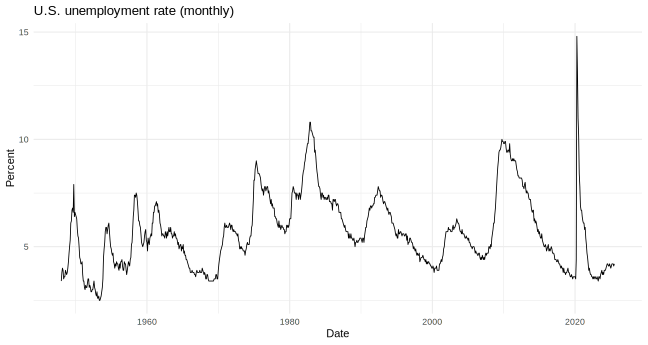
\includegraphics[width=0.95\textwidth]{figures/fig_unemployment_long.pdf}
\caption{U.S. unemployment rate, monthly.}
\label{fig:unemp}
\end{figure}

\begin{figure}[h]
\centering
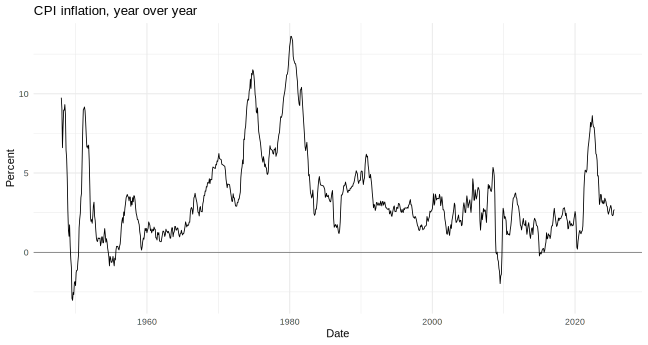
\includegraphics[width=0.95\textwidth]{figures/fig_inflation_cpi.pdf}
\caption{U.S. CPI inflation, year over year, monthly.}
\label{fig:infl}
\end{figure}

\subsection{Real GDP and detrending choices}

Figure \ref{fig:gdp-trend} plots $\log$ real GDP (GDPC1, quarterly) against four trend specifications. Figure \ref{fig:gdp-detrended} overlays the corresponding detrended series. Figure \ref{fig:gdp-cf} reports the Christiano-Fitzgerald decomposition into cycle, trend, and irregular components.

\begin{figure}[h]
\centering
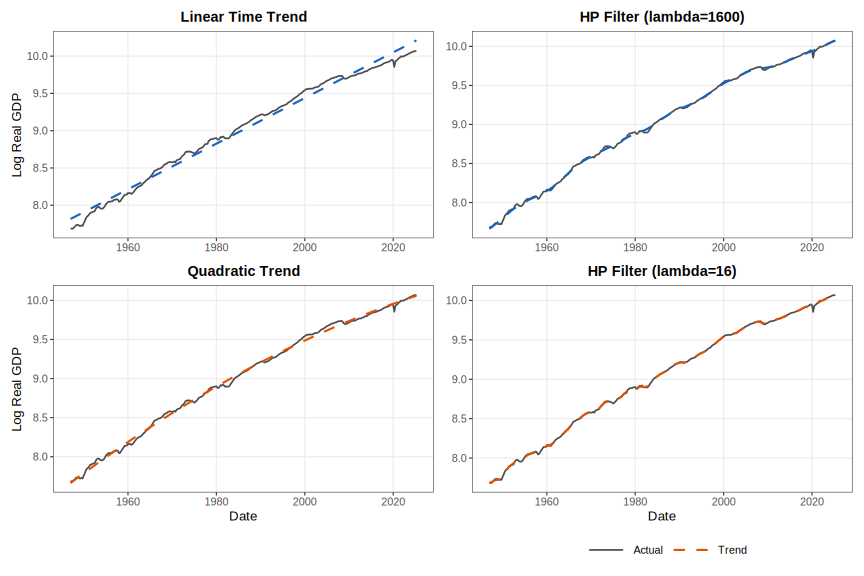
\includegraphics[width=0.98\textwidth]{figures/fig_gdp_trend_panels.pdf}
\caption{Log real GDP with linear, quadratic, and HP trends.}
\label{fig:gdp-trend}
\end{figure}

\begin{figure}[h]
\centering
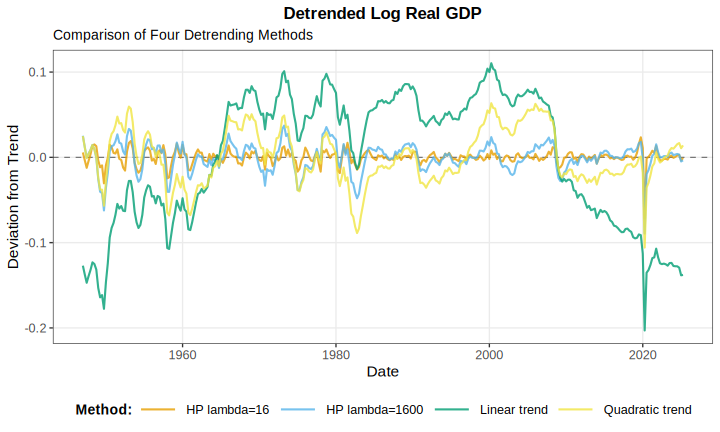
\includegraphics[width=0.75\textwidth]{figures/fig_gdp_detrended_overlay.pdf}
\caption{Detrended log real GDP under four detrending methods.}
\label{fig:gdp-detrended}
\end{figure}

\begin{figure}[h]
\centering
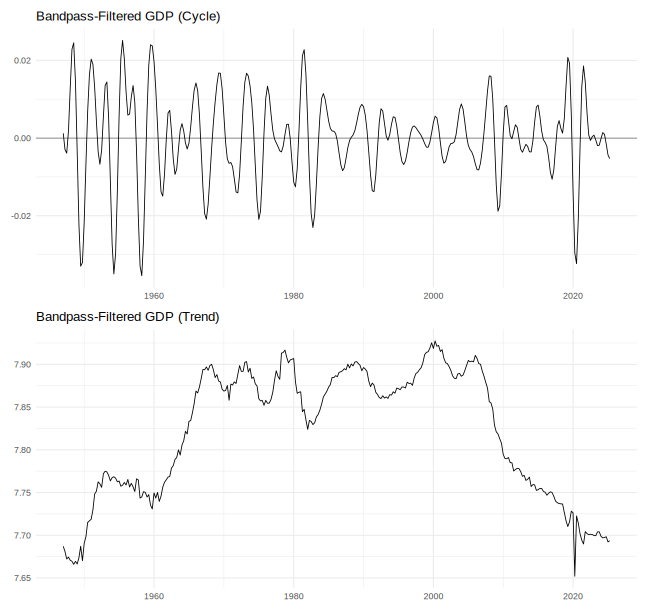
\includegraphics[width=0.80\textwidth]{figures/fig_gdp_cffilter_components.pdf}
\caption{Christiano-Fitzgerald bandpass decomposition of log real GDP.}
\label{fig:gdp-cf}
\end{figure}

\subsection{Impulse responses from univariate dynamics}

To illustrate how detrending affects dynamics, we fit AR models to the linear-detrended and quadratic-detrended log real GDP and report the implied impulse responses in Figure \ref{fig:irf-ar}.

\begin{figure}[h]
\centering
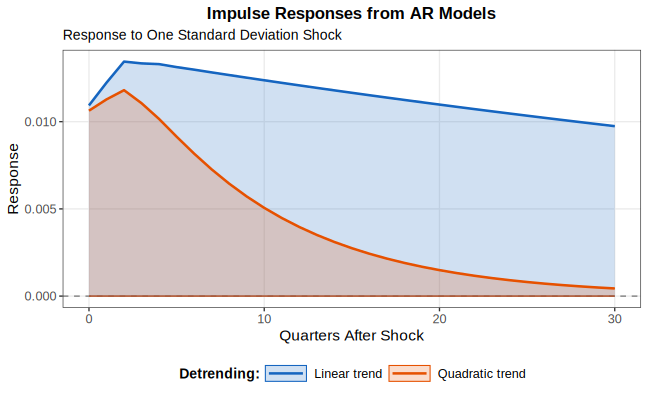
\includegraphics[width=0.72\textwidth]{figures/fig_irf_ar_linear_vs_quadratic.pdf}
\caption{Impulse responses from AR models estimated on linearly and quadratically detrended GDP.}
\label{fig:irf-ar}
\end{figure}

\subsection{Comovements with components of demand and labor market variables}

We compute cross-correlations between the cyclical component of output and the cyclical components of consumption, investment, inventories, exports, government purchases, hours, employment, inflation, the nominal rate, and the ex-post real rate. The table replicates the layout of Table 2 in the original note with leads and lags from $-6$ to $+6$ quarters. The R script writes a LaTeX table that is included below.

% Note: Table generation needs debugging - CF filter may not be producing valid cyclical components
% \begin{landscape}
% % latex table generated in R 4.5.1 by xtable 1.8-4 package
% Mon Sep  1 12:08:10 2025
\begin{table}[ht]
\centering
\caption{Cross-correlations of cyclical components with output, leads and lags -6..6 quarters. Std Dev is relative to cyclical GDP.} 
\label{tab:ccf}
\begin{tabular}{rrrrrrrrrrrrrrr}
  \hline
series & StdDev & -6 & -5 & -4 & -3 & -2 & -1 & 0 & 1 & 2 & 3 & 4 & 5 & 6 \\ 
  \hline
Average weekly hours &  &  &  &  &  &  &  &  &  &  &  &  &  &  \\ 
  Consumption &  &  &  &  &  &  &  &  &  &  &  &  &  &  \\ 
  Employment &  &  &  &  &  &  &  &  &  &  &  &  &  &  \\ 
  Ex-post real 10y rate &  &  &  &  &  &  &  &  &  &  &  &  &  &  \\ 
  Exports &  &  &  &  &  &  &  &  &  &  &  &  &  &  \\ 
  Federal funds rate &  &  &  &  &  &  &  &  &  &  &  &  &  &  \\ 
  Government purchases &  &  &  &  &  &  &  &  &  &  &  &  &  &  \\ 
  Inflation (GDP deflator) &  &  &  &  &  &  &  &  &  &  &  &  &  &  \\ 
  Inventory investment &  &  &  &  &  &  &  &  &  &  &  &  &  &  \\ 
  Investment &  &  &  &  &  &  &  &  &  &  &  &  &  &  \\ 
  Real wage &  &  &  &  &  &  &  &  &  &  &  &  &  &  \\ 
  S&P 500 &  &  &  &  &  &  &  &  &  &  &  &  &  &  \\ 
   \hline
\end{tabular}
\end{table}

% \end{landscape}

\subsection{Monetary policy and activity: updated VAR evidence}

Following the spirit of Christiano, Eichenbaum, and Evans, we estimate a monthly VAR on industrial production, the CPI, a commodity price index, the federal funds rate, total reserves, and M2, using a Cholesky identification that treats the federal funds rate as reacting within the month to the other variables. Figure \ref{fig:mp-irf} reports impulse responses to a 100 basis point innovation to the federal funds rate. The sample starts in 1965 and can extend beyond 2007 as M2 definitions remained more stable than M1.

\begin{figure}[h]
\centering
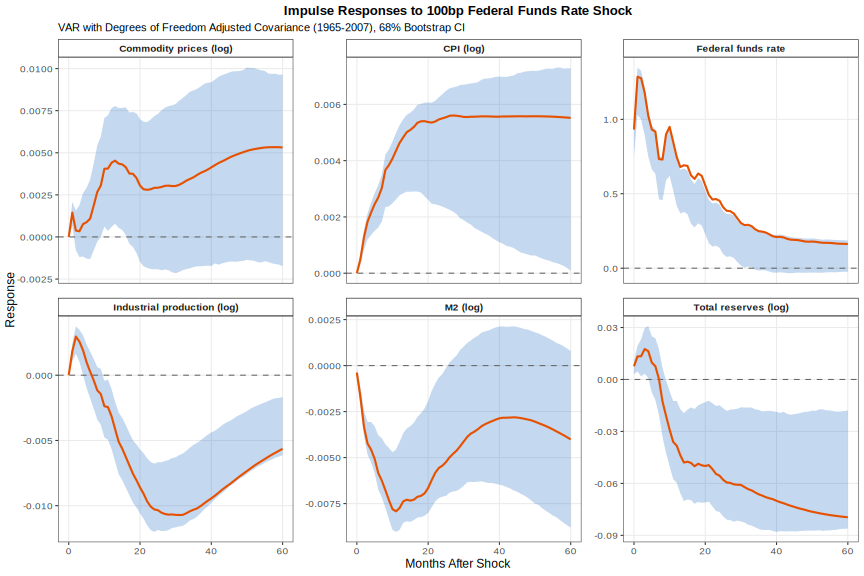
\includegraphics[width=0.98\textwidth]{figures/fig_mp_irf_grid.pdf}
\caption{Impulse responses to a 100 basis point federal funds rate shock from a monthly VAR.}
\label{fig:mp-irf}
\end{figure}

\section{Data and reproducibility} \label{sec:data}

All figures and the correlation table are reproducible by running the R script \texttt{make\_figures.R}. The script fetches series from FRED using \texttt{fredr} and writes graphics to \texttt{figures/} and a LaTeX table to \texttt{tables/}. Key FRED series used include

\begin{center}
\begin{tabular}{ll}
\toprule
Concept & FRED series ID \\
\midrule
Unemployment rate & UNRATE \\
Consumer Price Index & CPIAUCSL \\
Real GDP (chain, SAAR) & GDPC1 \\
Real PCE & PCEC96 \\
Real gross private domestic investment & GPDIC1 \\
Change in private inventories (real) & CBIC1 \\
Real exports of goods and services & EXPGSC1 \\
Real government consumption and investment & GCEC1 \\
Nonfarm payroll employment & PAYEMS \\
Average weekly hours, manufacturing & AWHMAN \\
Average hourly earnings, production and nonsupervisory & AHETPI \\
GDP implicit price deflator & GDPDEF \\
10-year Treasury constant maturity rate & GS10 \\
Industrial production index & INDPRO \\
Producer price index, all commodities & PPIACO \\
Federal funds rate & FEDFUNDS \\
Total reserves of depository institutions & TOTRESNS \\
M2 money stock & M2SL \\
S\&P 500 index & SP500 \\
\bottomrule
\end{tabular}
\end{center}

Users must set an environment variable \texttt{FRED\_API\_KEY} before running the script. The VAR sample starts in 1965 and uses M2 as the monetary aggregate to avoid definitional changes that affected M1 in 2020.

\section{Relation to the original figures}

The original note contains the trend-versus-cycle figures for log real GDP, a band-pass decomposition of GDP, a large correlation table across components, and impulse responses to monetary policy shocks, see pages 17 to 26 of the original PDF. The present document mirrors those elements with current data and with transparent code so that the figures can be refreshed. 

\end{document}